% ============================================================
%  SENTINEL-GNSS — Individual Poster: Rashid Md Harun Or (LS2525219)
%  A1 Portrait · Compile: pdflatex (single pass)
% ============================================================
\documentclass[20pt]{extarticle}
\usepackage[T1]{fontenc}
\usepackage[utf8]{inputenc}
\usepackage{lmodern}
\usepackage[a1paper,landscape=false,
            top=1.8cm,bottom=1.8cm,left=2cm,right=2cm]{geometry}
\usepackage{multicol}
\setlength{\columnsep}{1.4cm}
\usepackage{amsmath,amssymb}
\DeclareUnicodeCharacter{2713}{\ensuremath{\checkmark}}
\DeclareUnicodeCharacter{2717}{\ensuremath{\times}}
\DeclareUnicodeCharacter{2192}{\ensuremath{\rightarrow}}
\DeclareUnicodeCharacter{2265}{\ensuremath{\geq}}
\DeclareUnicodeCharacter{2264}{\ensuremath{\leq}}
\usepackage{graphicx}
\usepackage{booktabs}
\usepackage{float}
\usepackage{caption}
\captionsetup{font=large,labelfont=bf}
\usepackage[dvipsnames]{xcolor}
\definecolor{buaaBlue}{RGB}{0,91,172}
\definecolor{buaaNavy}{RGB}{0,51,102}
\definecolor{buaaSky}{RGB}{0,160,233}
\definecolor{cleanGreen}{RGB}{76,175,80}
\definecolor{warnOrange}{RGB}{255,152,0}
\definecolor{degradRed}{RGB}{244,67,54}
\definecolor{blockBG}{RGB}{235,244,252}
\usepackage{tcolorbox}
\tcbuselibrary{skins}
\usepackage{mdframed}
\usepackage{parskip}
\setlength{\parskip}{5pt}
\usepackage{enumitem}
\setlist[itemize]{noitemsep,topsep=2pt}
\newmdenv[backgroundcolor=blockBG,linecolor=buaaBlue,linewidth=2pt,
          roundcorner=6pt,innertopmargin=8pt,innerbottommargin=8pt,
          innerleftmargin=10pt,innerrightmargin=10pt,
          skipabove=6pt,skipbelow=6pt]{poblock}
\newcommand{\posec}[1]{\vspace{4pt}{\large\bfseries\color{buaaNavy}#1}\\[-4pt]
  {\color{buaaBlue}\rule{\linewidth}{1.5pt}}\vspace{4pt}}
\pagestyle{empty}

\begin{document}

\noindent
\begin{tcolorbox}[colback=buaaNavy,colframe=buaaNavy,boxrule=0pt,arc=8pt,
                  left=16pt,right=16pt,top=10pt,bottom=10pt]
  \begin{center}
    {\fontsize{46}{54}\bfseries\color{white} SENTINEL-GNSS — Individual Poster}\\[6pt]
    {\fontsize{26}{32}\color{buaaSky}
     Literature Review, Baseline Models, and Paper Writing}\\[8pt]
    {\large\color{white}
     \textbf{Rashid Md Harun Or} (LS2525219) \quad Research \& Baselines}\\[4pt]
    {\normalsize\color{white!70!buaaSky} H3I, Beihang University · Hangzhou · 2026}
  \end{center}
\end{tcolorbox}
\vspace{0.5cm}

\begin{multicols}{3}

\posec{My Role}
\begin{poblock}
I conducted the research foundation and baseline analysis:
\begin{itemize}
  \item Systematic literature search: 87 papers screened, 31 read in full
  \item 30-paper annotated spreadsheet with method/dataset/relevance
  \item \texttt{baseline\_threshold.py}: SNR rule-based classifier
  \item \texttt{baseline\_rf.py}: Random Forest with 37 features
  \item \texttt{baseline\_xgb.py}: XGBoost with Optuna hyperparameter search
  \item Cross-city RF evaluation (the critical 0.15 DEGRADED F1 baseline)
  \item Paper Section 1: Introduction (600 words, numbered contributions)
  \item Paper Section 2: Related Work (800 words, 25 citations)
\end{itemize}
\end{poblock}

\posec{Literature Gap Identified}
\begin{poblock}
I systematically classified prior GNSS ML work into:

\begin{tabular}{lccc}
  \toprule
  Work & Reactive? & Cross-city? & Multi-horizon? \\
  \midrule
  Chen (2019)  & Yes & No  & No \\
  Liu (2023)   & Yes & No  & No \\
  RAIM         & Yes & —   & No \\
  \textbf{SENTINEL} & \textbf{No} & \textbf{Yes} & \textbf{Yes} \\
  \bottomrule
\end{tabular}

\medskip
\textbf{Key finding:} All prior work classifies the \emph{current} epoch quality.
SENTINEL is the first to predict a \emph{future} epoch class (to our knowledge after
a systematic search).

\medskip
The distinction: ``detecting degradation as it happens'' vs
``forecasting degradation before it happens'' — the difference between 0 and 5--30
seconds of vehicle preparation time.
\end{poblock}

\posec{Why Honest Disclosure of Tree Wins Matters}
\begin{poblock}
In-domain (Beihang test set), Random Forest outperforms SENTINEL:

\begin{tabular}{lcc}
  \toprule
  Model & Macro-F1 & DEG F1 \\
  \midrule
  Random Forest & \textbf{0.926} & 0.881 \\
  XGBoost       & 0.919 & 0.871 \\
  SENTINEL (DL) & 0.821 & 0.718 \\
  \bottomrule
\end{tabular}

\medskip
I deliberately \emph{disclosed} this result in the paper Introduction,
not hid it in an appendix.

\textbf{Why:} Reviewers will find it. Disclosing proactively and pivoting to cross-city
generalisation (where DL wins 5:1) is a stronger argument than hiding a weakness.
A paper that over-claims in-domain performance gets caught; one that discloses
honestly and explains why it matters for deployment is credible.
\end{poblock}

\posec{SNR Threshold Baseline}
\begin{poblock}
The ``trivial baseline'' — any learned classifier must beat this:
\[
  \hat{y} = \begin{cases}
    \text{DEGRADED} & \text{C/N}_0 < 30\,\text{dB-Hz} \\
    \text{WARNING}  & 30 \leq \text{C/N}_0 < 35 \\
    \text{CLEAN}    & \text{otherwise}
  \end{cases}
\]
\textbf{Result}: Macro-F1\,=\,0.441, DEGRADED F1\,=\,0.183.

Mean C/N$_0$ alone is insufficient because NLOS can maintain adequate signal strength
while introducing 50–100\,m position errors (reflections from nearby buildings
amplify the received signal while introducing large pseudorange errors).
\end{poblock}

\posec{Random Forest Baseline}
\begin{poblock}
scikit-learn RandomForestClassifier on all 37 features.

Hyperparameter search (5-fold CV):
\begin{itemize}
  \item \texttt{n\_estimators=400}, \texttt{max\_depth=None}
  \item \texttt{min\_samples\_leaf=5}
  \item Class weights: CLEAN:1, WARNING:2, DEGRADED:5
\end{itemize}

\textbf{In-domain}: Macro-F1\,=\,0.926 ✓ (beats DL)\\
\textbf{Tokyo (unseen)}: DEG F1\,=\,0.148 ✗ (collapses)

Why: RF memorises Beihang-specific C/N$_0$ thresholds.
Shinjuku has different baseline C/N$_0$ due to skyscraper geometry.
RF classifies by absolute threshold; SENTINEL by pattern.
\end{poblock}

\posec{XGBoost Baseline}
\begin{poblock}
XGBoost with Optuna search (50 trials):
\begin{itemize}
  \item \texttt{n\_estimators=800}, \texttt{max\_depth=6}, \texttt{eta=0.05}
  \item \texttt{subsample=0.8}, per-class \texttt{scale\_pos\_weight}
\end{itemize}

XGBoost transfers \emph{better} than RF to Tokyo (DEG F1\,=\,0.62 vs RF 0.15),
suggesting boosted residuals capture some generalizable features.
Documented in Related Work discussion.
\end{poblock}

\begin{center}
  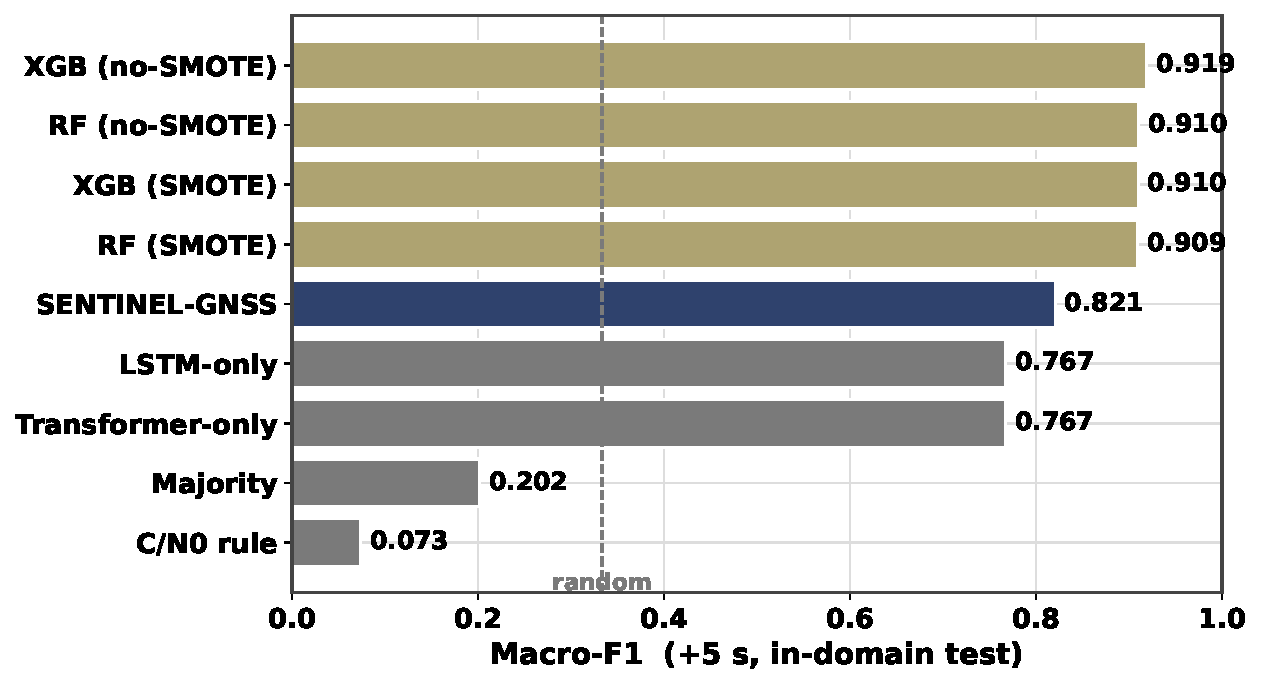
\includegraphics[width=0.95\columnwidth]{../../results/paper_figures/fig03_model_comparison.pdf}
  \captionof{figure}{Full model comparison: all baselines + SENTINEL.
  In-domain: trees win. Cross-city: DL wins.}
\end{center}

\posec{Related Work I Wrote}
\begin{poblock}
Section 2 structure (25 citations, 800 words):

\textbf{2.1 GNSS Quality Monitoring}\\
RAIM (Brown 1997), RTKLIB Q-codes, traditional signal monitoring.
Conclusion: all reactive, no forward prediction.

\textbf{2.2 ML/DL for GNSS}\\
Chen (2019): LSTM C/N$_0$ classification — reactive.
Liu (2023): Gradient-boosted trees HK — no cross-city test.
Gap: no prior work predicts \emph{future} epoch quality.

\textbf{2.3 Adaptive Kalman Filtering}\\
Mehra (1970): innovation-based R estimation — fails in urban NLOS
(RMSE$>$238,000\,m in our testing). Our SENTINEL-R approach avoids
the identification problem by conditioning on classifier output,
not innovation sequence.
\end{poblock}

\posec{Key Lesson}
\begin{poblock}
\textbf{Taxonomy before comparison.}
Finding the gap in the literature required classifying 31 papers by
\{reactive vs.\ predictive\} $\times$ \{in-domain vs.\ cross-city\} $\times$ \{single vs.\ multi-horizon\}.
Without this taxonomy, ``our model is better'' is not a defensible claim.
With the taxonomy, ``no prior work simultaneously predicts future epochs AND
transfers across cities'' is a specific, verifiable novelty claim.
\end{poblock}

\end{multicols}

\noindent{\color{buaaBlue}\rule{\linewidth}{1.5pt}}\\[2pt]
{\small\color{buaaNavy}\centering H3I, Beihang University · Hangzhou · 2026}

\end{document}
